\documentclass{article}[jsarticle]
\usepackage[T1]{fontenc}
\usepackage[dvipdfmx]{hyperref}
\usepackage{lmodern}
\usepackage{latexsym}
\usepackage{amsfonts}
\usepackage{amssymb}
\usepackage{mathtools}
\usepackage{nccmath}
\usepackage{amsthm}
\usepackage{multirow}
\usepackage{graphicx}
\usepackage[dvipdfmx]{color}
\usepackage{wrapfig}
\usepackage{here}
\usepackage{float}
\usepackage{ascmac}
\usepackage{url}
\usepackage{listings}
\usepackage{xcolor}

\lstset{
    basicstyle=\ttfamily\color{white},
    numbers=none,  % Line numbers
    numberstyle=\tiny\color{white},
    numbersep=5pt,
    tabsize=2,
    extendedchars=true,
    breaklines=true,
    keywordstyle=\color[rgb]{0.58,0.00,0.83},
    stringstyle=\color[rgb]{0.81,0.36,0.00},
    identifierstyle=\color{white},
    commentstyle=\color[rgb]{0.34,0.62,0.16},
    rulecolor=\color[rgb]{0.5,0.5,0.5},
    xleftmargin=0.1cm,    % Left margin
    xrightmargin=0.1cm,   % Right margin
    language=python,
    backgroundcolor=\color[rgb]{0.13,0.13,0.13},
    showspaces=false,
    showstringspaces=false
}



\title{機械学習 課題1}
\author{高林秀 \\ 三宅研究室 博士前期課程1年 \\ V-CampusID : 23vr008n}
\date{\today}

\begin{document}

\maketitle

\begin{abstract}
    \noindent
    本稿は本年度必修授業の機械学習の第1回レポートの答案用紙である。\par
    \noindent
    本稿は、第1回授業~第4回授業までの範囲を対象とし、各回で課された課題に対する解答を記載する。\par
    \noindent
    答案の問題番号は各章のタイトルに記載している。\par
    \noindent
    各問に対する解答は本稿に、コードなどの実行結果は別途GoogleColaboratoryのノートブックに記載した
    巻末の付録から参照できる。
\end{abstract}

\section{第1回授業 : 4/11 宿題1}
    \subsection{問題文}
    二つのデータ点の近さを測る定量的指標の一つとして距離がある。いま、次の三つのデータ点があるとする
    \begin{flalign}
        & \text{データ点1} : (5,2,5.8) \\
        & \text{データ点2} : (7, 10, 1, 12) \\
        & \text{データ点3} : (3, 2, 6, 3)
    \end{flalign}
    上の各データ点は4種類の計測値で与えられている(例えば「緯度、経度、水深、温度」のような感じ)。
    このデータ点同士の間の近さをユークリッド距離で計算し、互いの距離が近いペアの順番を答えよ。データが近いほど距離が小さいことに注意。
    
    \subsection{解答}
    データ点の近さは以下の順番である。
    \begin{enumerate}
        \item データ点1とデータ点3、距離 : $5.4$
        \item データ点1とデータ点2、距離 : $10.0$
        \item データ点2とデータ点3、距離 : $13.6$
    \end{enumerate}
    ユークリッド距離は以下の式で計算できる。
    \begin{flalign*}
        & d(x,y) :\text{データ点xとデータ点yの距離として、}\\
        & d(x,y) = \sqrt{\sum_{i=1}^{n}(x_i - y_i)^2} \\
        & \text{※}x_i,y_i\text{はそれぞれデータ点}x,y\text{のi番目の要素を表す}
    \end{flalign*}
    各点間の距離は以下のように計算できる %TODO:後で手計算すること
    \begin{flalign*}
        & d(1,3) = \sqrt{(5-3)^2 + (2-2)^2 + (5.8-6)^2 + (0-3)^2} = 5.4 \\
        & d(1,2) = \sqrt{(5-7)^2 + (2-10)^2 + (5.8-1)^2 + (0-12)^2} = 10.0 \\
        & d(2,3) = \sqrt{(7-3)^2 + (10-2)^2 + (1-6)^2 + (12-3)^2} = 13.6
    \end{flalign*}

\section{第2回授業 : 4/18 宿題2}% TODO:PrecisionとRecallを再計算すること
    \subsection{問題文}
    \begin{figure}[H]
        \centering
        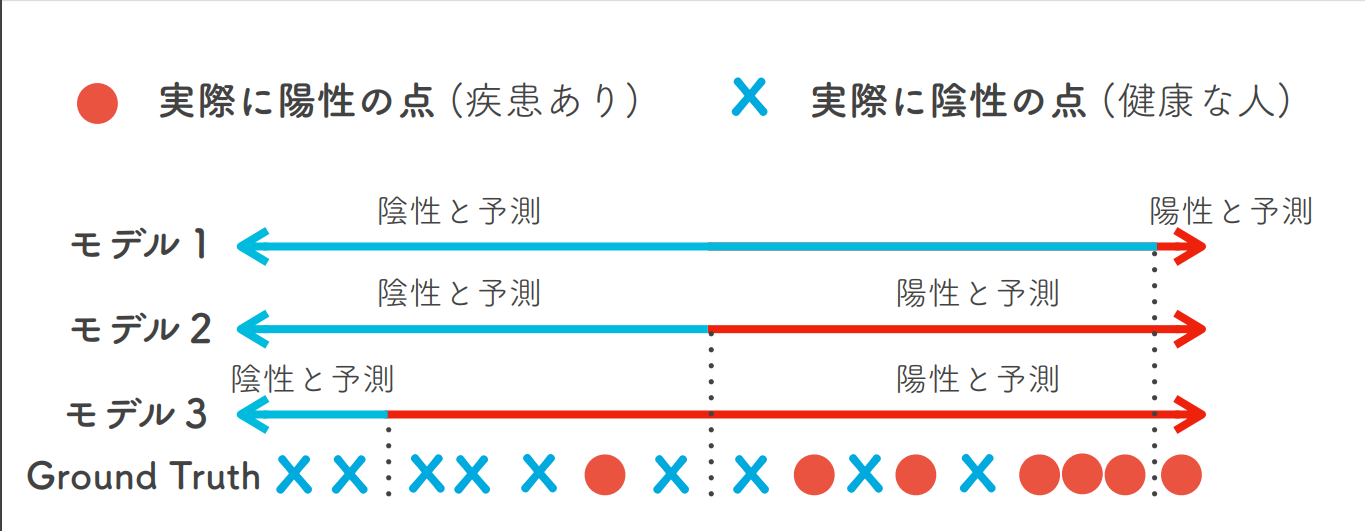
\includegraphics[scale=0.7]{./images/MLQ2.png}
    \end{figure}
    \begin{enumerate}
        \item 上の三つの分類モデルそれぞれに対し、混同行列、Precision、Recallを計算しなさい。
        \item モデル1→モデル2→モデル3の順に、Precisionは増加や減少の傾向にあるでしょうか?その傾向はなぜ生じるでしょう?また、Recallについても傾向はどうなっていますか?Precisionの傾向と対比して議論して見てください。
    \end{enumerate}
    
    \subsection{解答:問1}
    まず、各モデルの混同行列とPrecision、Recallを計算した結果は以下のようになる。
    \subsubsection{モデル1}
    % Please add the following required packages to your document preamble:
% \usepackage{multirow}
    \begin{table}[H]
        \centering
        \begin{tabular}{llcc}
                                                                        & \multicolumn{1}{l|}{}   & \multicolumn{2}{c}{予測}                         \\
                                                                        & \multicolumn{1}{l|}{}   & \multicolumn{1}{c|}{陽性} & 陰性                   \\ \hline
        \multirow{2}{*}{\begin{tabular}[c]{@{}l@{}}実\\ データ\end{tabular}} & \multicolumn{1}{c|}{陽性} & \multicolumn{1}{c|}{1}  & 6                    \\ \cline{2-4} 
                                                                        & \multicolumn{1}{c|}{陰性} & \multicolumn{1}{c|}{0}  & 9                    \\
                                                                        &                         & \multicolumn{1}{l}{}    & \multicolumn{1}{l}{}
        \end{tabular}
        \caption{モデル1の混同行列}
    \end{table}
    \begin{itemize}
        \centering
        \item Precision : $\frac{TP}{TP + FP} = \frac{1}{1 + 0} = 1.0$
        \item Recall : $\frac{TP}{TP + FN} = \frac{1}{1 + 6} = \frac{1}{7} \approx 0.14$
    \end{itemize}

    \subsubsection{モデル2}
    % Please add the following required packages to your document preamble:
    % \usepackage{multirow}
    \begin{table}[H]
        \centering
        \begin{tabular}{llcc}
                                                                        & \multicolumn{1}{l|}{}   & \multicolumn{2}{c}{予測}                         \\
                                                                        & \multicolumn{1}{l|}{}   & \multicolumn{1}{c|}{陽性} & 陰性                   \\ \hline
        \multirow{2}{*}{\begin{tabular}[c]{@{}l@{}}実\\ データ\end{tabular}} & \multicolumn{1}{c|}{陽性} & \multicolumn{1}{c|}{6}  & 1                    \\ \cline{2-4} 
                                                                        & \multicolumn{1}{c|}{陰性} & \multicolumn{1}{c|}{3}  & 6                    \\
                                                                        &                         & \multicolumn{1}{l}{}    & \multicolumn{1}{l}{}
        \end{tabular}
        \caption{モデル2の混同行列}
    \end{table}
    \begin{itemize}
        \centering
        \item Precision : $ \frac{6}{6 + 3} = \frac{2}{3}  \approx 0.67$
        \item Recall : $ \frac{6}{6 + 1} = \frac{6}{7} \approx 0.86$
    \end{itemize}

    \subsubsection{モデル3}
   % Please add the following required packages to your document preamble:
    % \usepackage{multirow}
    \begin{table}[H]
        \centering
        \begin{tabular}{llcc}
                                                                        & \multicolumn{1}{l|}{}   & \multicolumn{2}{c}{予測}                         \\
                                                                        & \multicolumn{1}{l|}{}   & \multicolumn{1}{c|}{陽性} & 陰性                   \\ \hline
        \multirow{2}{*}{\begin{tabular}[c]{@{}l@{}}実\\ データ\end{tabular}} & \multicolumn{1}{c|}{陽性} & \multicolumn{1}{c|}{7}  & 0                    \\ \cline{2-4} 
                                                                        & \multicolumn{1}{c|}{陰性} & \multicolumn{1}{c|}{7}  & 2                    \\
                                                                        &                         & \multicolumn{1}{l}{}    & \multicolumn{1}{l}{}
        \end{tabular}
        \caption{モデル3の混同行列}
    \end{table}
    \begin{itemize}
        \centering
        \item Precision : $ \frac{7}{7 + 7} = \frac{1}{2} = 0.5$
        \item Recall : $ \frac{7}{7 + 0} = 1.0$
    \end{itemize}

    \subsection{解答:問2}
    計算結果から、Precision(適合率)は減少の傾向にあるといえる。Precisionは、陽性と予測したデータ数のうち、実際に陽性だったデータ数の割合を示す。計算式で示すと以下の通り。
    \begin{flalign*}
        & Precision = \frac{TP}{TP + FP} \\
        & \text{※}TP\text{は真陽性、FPは偽陽性を表す}
    \end{flalign*}
    この式より、Precisionは分母の、モデルが陽性と予測した数が少なければ値が大きくなる傾向にあることがわかる。
    モデル1では陽性と予測されたデータ数は$1$で、モデル2では$9$、モデル3では$14$と徐々に陽性予測のデータ数が増えており、Precisionの式の分母が大きくなっているので、
    モデル1~モデル3にかけてPrecisionは減少していると考えられる。\par

    また、Recall(再現率)は増加の傾向にあるといえる。Recallは、実際に陽性だったデータのうち、モデルが正しく陽性と予測したデータ数の割合を示す。計算式で示すと以下の通り。
    \begin{flalign*}
        & Recall = \frac{TP}{TP + FN} \\
        & \text{※}TP\text{は真陽性、FNは偽陰性を表す}
    \end{flalign*}
    この式より、Recallは分母の、実際は陽性だが予測では陰性だった割合が少ないほどRecallは大きくなる傾向にあることがわかる。
    実際は陽性だったデータのうち、モデルが陰性と予測したデータの割合がモデル1~モデル3にかけて減少したことから、Recallは増加していると考えられる。\par


\section{第3回授業 : 4/25 宿題1}
    \subsection{問題文}
    Xの数値スケールが大きく(例えば0~1000000)、Yのスケールが小さい(例えば0~1)データに対して、スケーラを使わないで回帰をしたとする。
    \begin{enumerate}
        \item 勾配降下法で学習率を大きくしても小さくしても問題が起こることを説明せよ。
        \item パラメータ$a, b$ごとに学習率を変えて勾配降下法をすれば、スケーラを使わなくても 1. の問題は抑制できるか?具体的な誤差関数の形を使って議論せよ。
    \end{enumerate}

    \subsection{解答:問1}
    特徴量の間のスケールの差が大きい場合、勾配降下法実行時に行われるパラメータの更新幅が、パラメータによって偏りが生じるという現象が生じる。
    つまり、パラメータのスケールが異なる場合、学習率の大小に関係なく、勾配の進み幅(パラメータの更新幅)がバラバラになる。
    その結果、最適解に収束しないことがあるので、スケーラーを使わない場合よりも、学習を完了するまで時間が長くなったり、モデルの精度が悪くなるという問題がある。\par 
    \noindent
    この問題はなぜ生じるのか、それはパラメータの更新幅が、特徴量の大きさに依存するからである。
    勾配降下法では、パラメータの更新幅は以下の式で表される。
    \begin{flalign*}
        & \theta_{new} = \theta_{old} - \eta \frac{\partial E(\theta)}{\partial \theta} \\
        & \text{※}E(\theta)\text{は誤差関数、}\eta\text{は学習率を表す}
    \end{flalign*}
    この式より、パラメータの更新幅は、学習率と誤差関数の勾配の積に比例することがわかる。
    ゆえに、誤差関数の勾配は、特徴量の大きさに依存し、特徴量の大きさ・スケールが異なる場合、誤差関数の勾配も異なる。
    そのため、特徴量のスケールが異なる場合、パラメータの更新幅も異なるため、最適解に収束しないことがある。\par

    \subsection{解答:問2}
    結論を先に考えれば、スケーラーを使わなくても、パラメータ毎に学習率を設定できればこの問題は抑止できるはずである。
    具体的な誤差関数として平均2乗誤差を用いた場合、
    \begin{flalign*}
       & \hat{y}_{i} = ax_{i} + b \\
       & MSE(a,b) = \frac{1}{n}\sum_{i=1}^{n}(y_i - \hat{y_i})^2
    \end{flalign*}
    これを等高線プロットした図を以下のURLから引用する。   
    \begin{figure}[H]
        \centering
        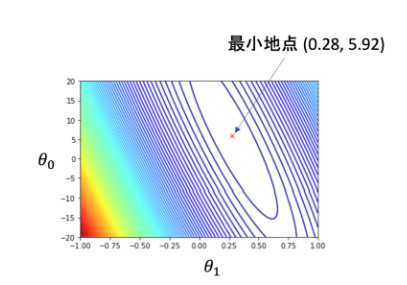
\includegraphics[scale=1.9]{./images/MSEGraph.png}
        \caption{
            MSEの等高線プロット, $\theta_0 = b, \theta_1 = a$と読み替えてください. \\
            【引用元】:米国データサイエンティストのブログ~損失関数の可視化 2022.02.16
        }
        \url{https://datawokagaku.com/cost_function/}
    \end{figure}
    この図からわかるように、パラメータ$a$と$b$の方向に対し、それぞれ異なる勾配を持っていることが分かる。
    学習率とは、勾配をどれだけの幅で更新するかを決めるハイパーパラメータである。ゆえに、パラメータ毎に学習率を設定することができれば、
    パラメータ毎に適切な勾配の進み幅、すなわちパラメータの更新幅を制御できるはずなので、スケーラーを用いずともこの問題は抑止できると考えられる。

    現にそのような観点から最適化を図る手法として、Adamなどの適応学習率と呼ばれる、勾配の大きさに従って適切な学習率を設定できる手法も提案されている。


\section{第4回授業 : 5/9 宿題1}
    \subsection{問題文}
    $R^2$ によるscore計算をNumpyを用いて実装して見ましょう(sklearnの出来合いの関数を使ってはいけません)。R2の定義式は講義のスライド参照。

    \subsection{解答}
    授業資料のノートブックに以下の関数を作成し、テストコードを実行した。そのコードと結果を以下に示す。
    \begin{lstlisting}
        from numpy import ndarray
        import numpy as np
        
        def r_square(y_hat: ndarray, y: ndarray):
        
          avg_y = (1/y.size) * y.sum()
          error_sq = np.square(y_hat - y)
          
          residual = error_sq.sum()
          totalSquares = (np.square(avg_y - y)).sum()
        
          return 1 - (residual / totalSquares)
        
        
        # 実際の値と予測値の生成
        y = np.array([1, 2, 3, 4, 5])
        y_hat = np.array([1.1, 1.9, 3.2, 3.7, 5.1])
        
        # $R^2$スコアの計算
        r2_score = r_square(y_hat, y)
        
        print(f"R^2 Score: {r2_score}")
        #R^2 Score: 0.984
    \end{lstlisting}
        
        

\section{付録}
各課題のコード(notebook形式)は、下記リンクのGoogleDriveフォルダに格納している。ノートブックのファイル名は\textbf{23vr008n-Report1.ipynb}。
\begin{itemize}
    \item 提出用GoogleDriveフォルダ
    \begin{itemize}
        \item \url{https://drive.google.com/drive/folders/1DZd7YFLM37_FVvvhxdTS5-6y9YXI4ulB?usp=drive_link}
    \end{itemize}
\end{itemize}
\end{document}